\documentclass{beamer-control}
\usepackage{beamer-control-singlefile}
\INCLUDEONLY{Examples}
\begin{document}
\CONCEPT{Examples}

\begin{SUMMARY}
\begin{itemize}
\item Cruise Control
\item Bicycle Dynamics
\end{itemize}
\vfill References:
\begin{itemize}
\item \astrom{Chapter 4}
\end{itemize}
\end{SUMMARY}



\SUBCONCEPT{Cruise Control}

\begin{frame}{Block diagram}
\vfill

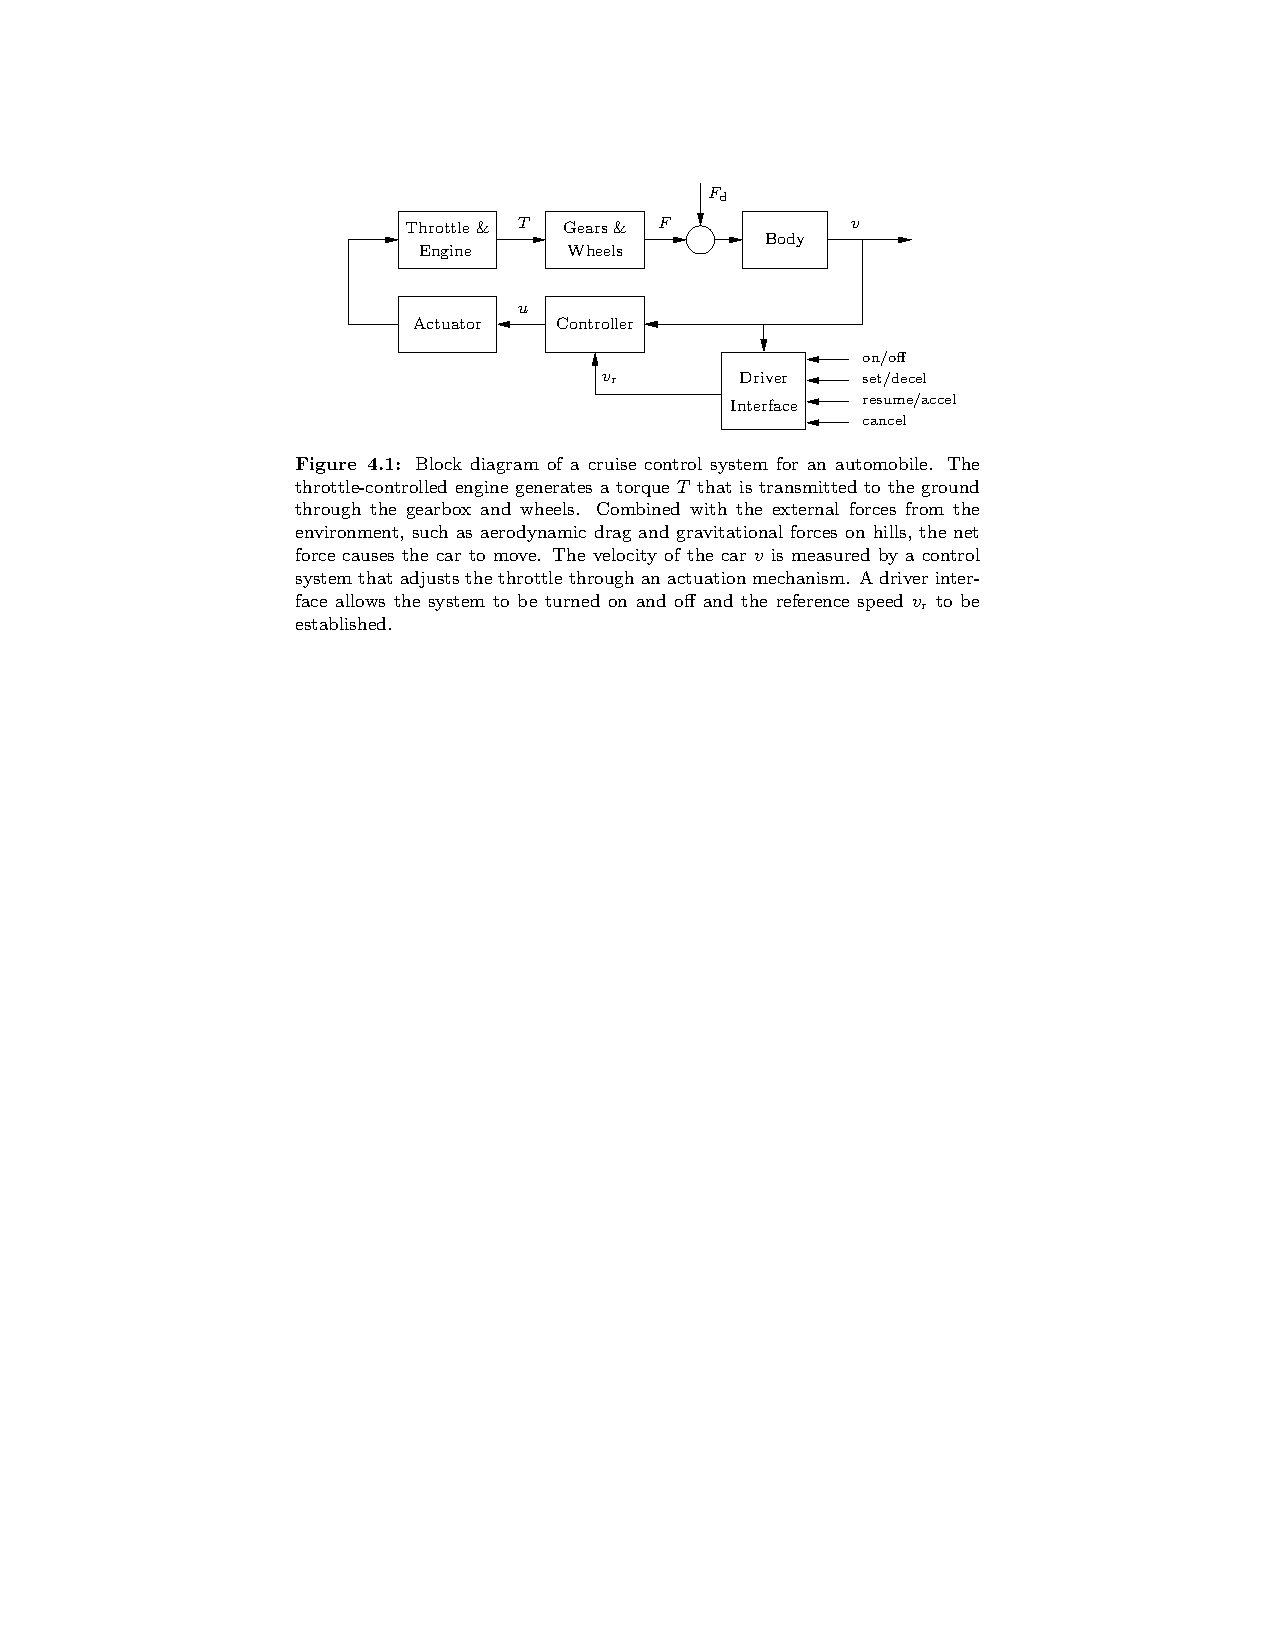
\includegraphics[width=\linewidth,clip,trim=0 65 0 0]{figure4.1}

\end{frame}

\begin{frame}{Modelling}{Free body diagram}
\begin{align}
\sum F &= m\ddot x = m\dot v \\
m\dot v &= uf - F_d
\end{align}
\begin{uncoverenv}<2->
\begin{align}
f &= \alpha_n T(\underbrace{\alpha_n v}_{\omega}) \\
T(\omega) &= T_m \biggl( 1 - \beta\Bigl(\frac{\omega}{\omega_m}-1\Bigr)^2 \biggr)
\end{align}
\end{uncoverenv}
\begin{uncoverenv}<3->
\begin{align}
F_d = F_r + F_a + F_g = \underbrace{mg C_r \operatorname{sgn}(v)}_{\text{friction}} + \underbrace{\tfrac12 \rho C_dA|v|v}_{\text{drag}} + \underbrace{mg\sin\theta}_{\text{gravity}}
\end{align}
\end{uncoverenv}
\end{frame}

\begin{frame}
\frametitle{Torque--speed graph}
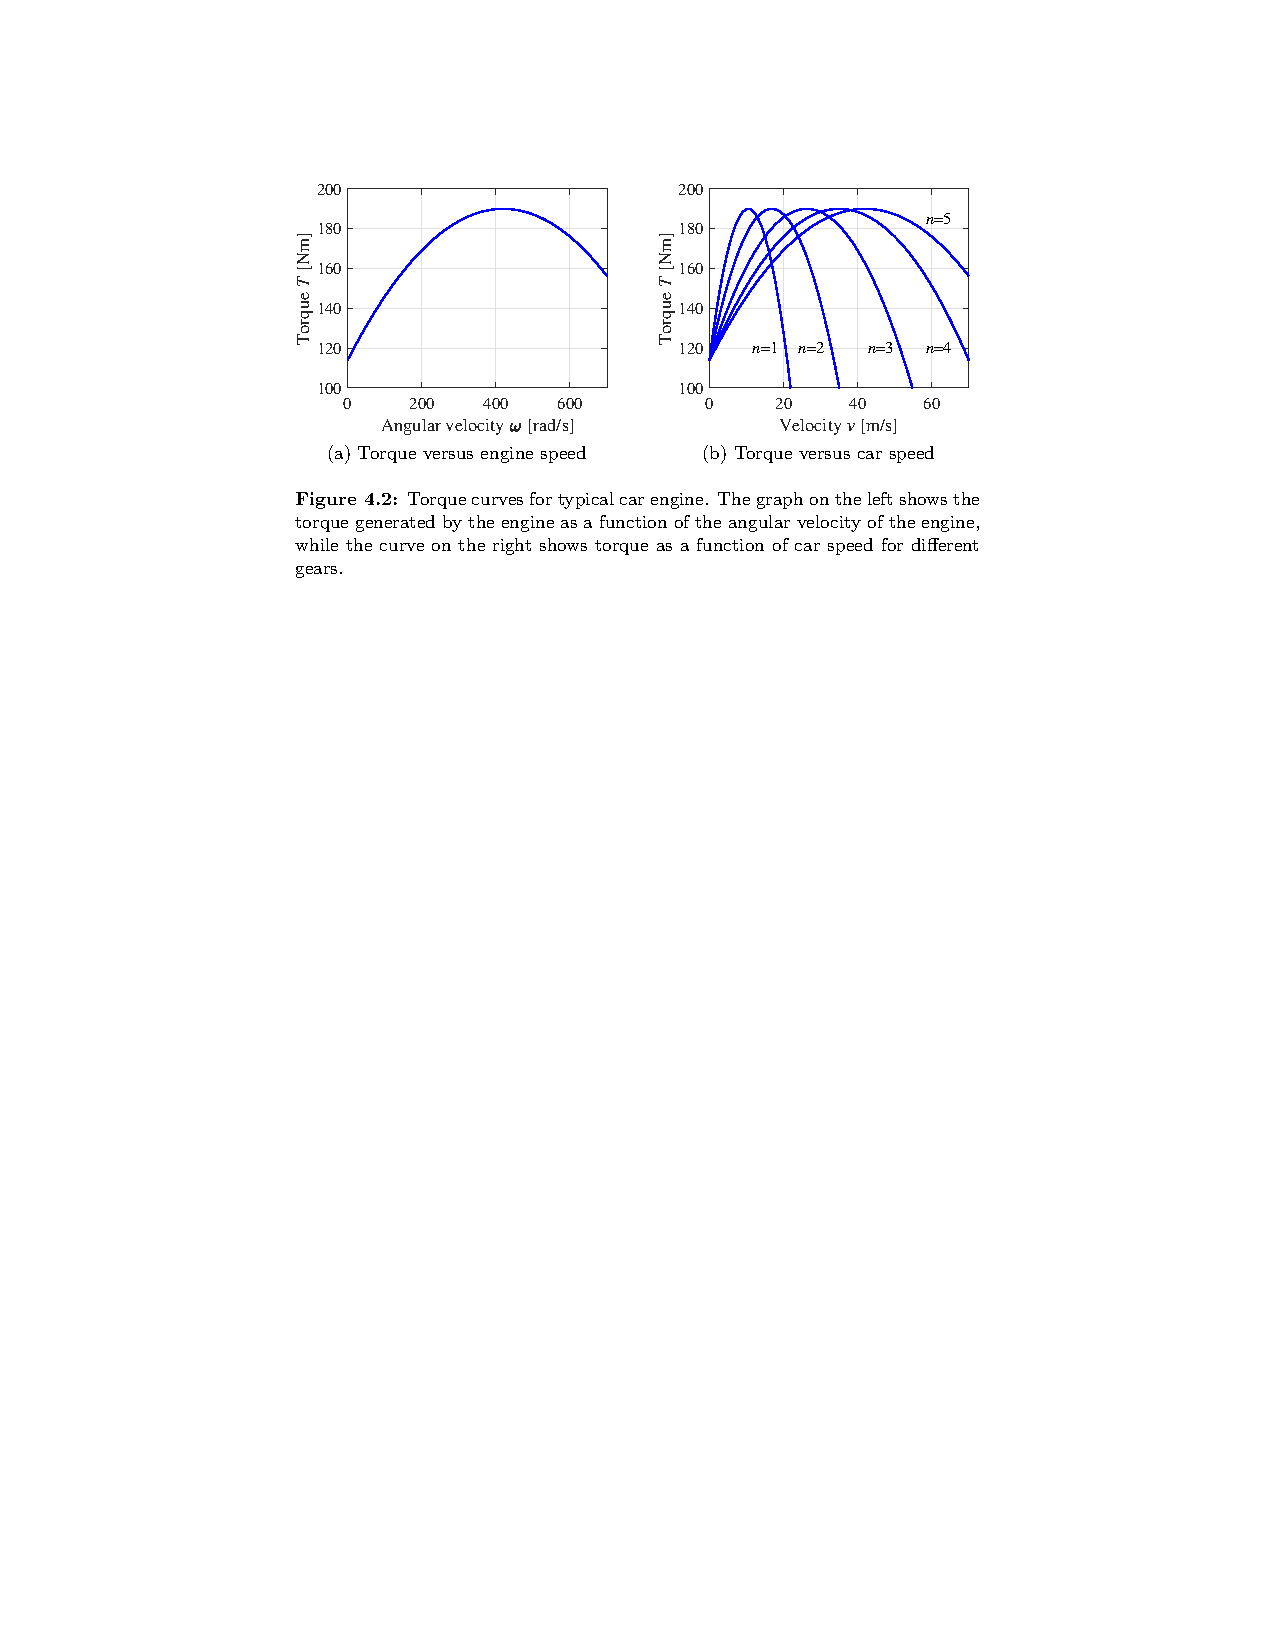
\includegraphics[width=\linewidth]{figure4.2}

\end{frame}

\begin{frame}
\frametitle{Force--speed graph}
\centering
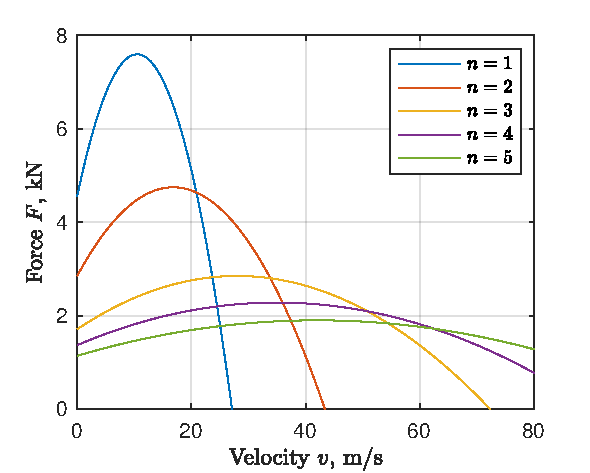
\includegraphics[scale=0.85]{pdf/car-fv}

\end{frame}

\begin{frame}
\frametitle{Steady state response --- 100\% throttle}
\includegraphics<1->[width=0.45\linewidth]{pdf/cruise-v0}\hfil
\includegraphics<2>[width=0.45\linewidth]{pdf/cruise-t0}
\end{frame}

\begin{frame}
\frametitle{Steady state response --- varying throttle}
\framesubtitle{Note the nonlinearity!}

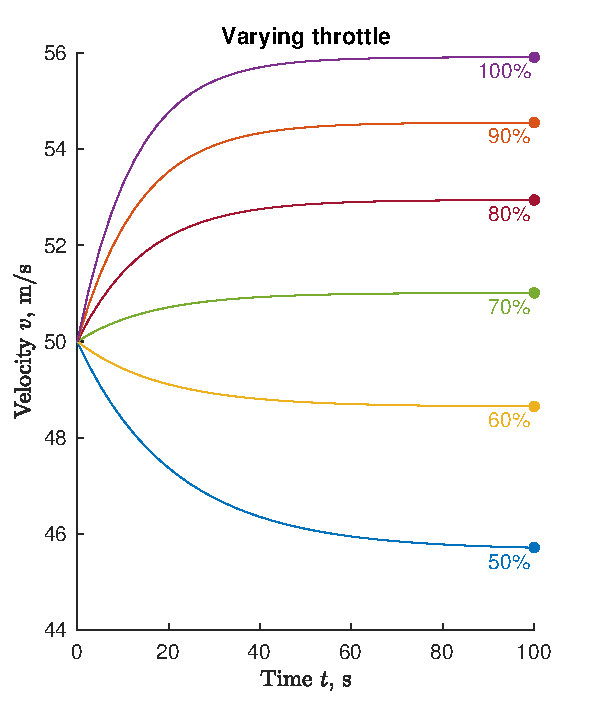
\includegraphics[width=0.45\linewidth]{pdf/cruise-u}\hfil
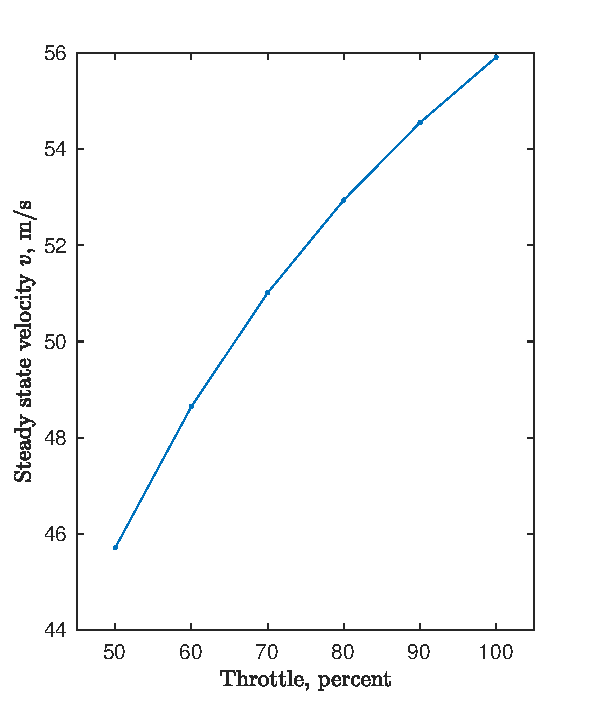
\includegraphics[width=0.45\linewidth]{pdf/cruise-uv}
\end{frame}

\begin{frame}
\frametitle{A kind of phase portrait}
\framesubtitle{A single condition is trivial, as this has 1DOF --- $\therefore$ plot multiple conditions}

\centering
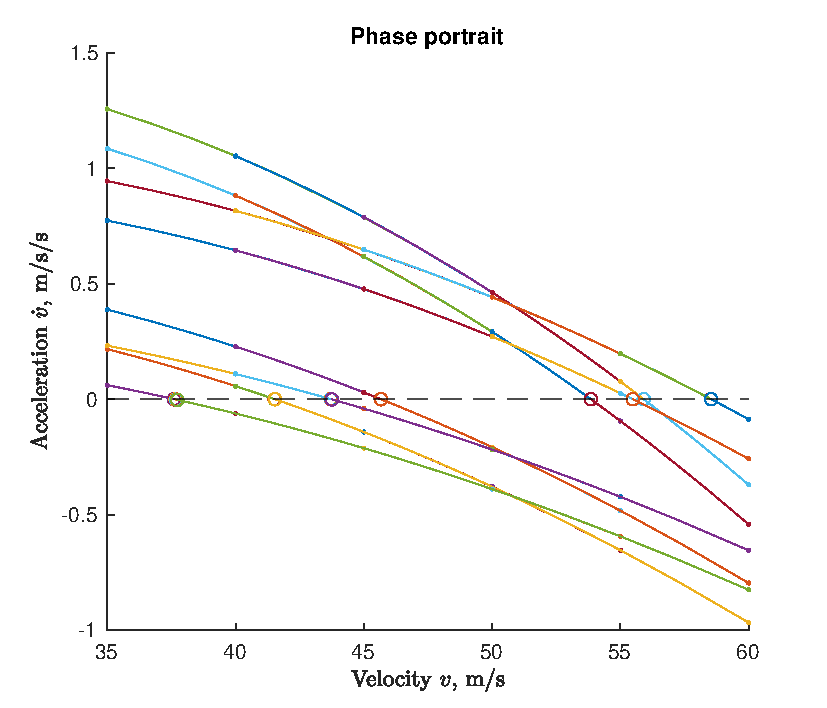
\includegraphics[height=0.9\textheight]{pdf/cruise-phase}

\QUIZ{Is this system stable in the sense of Lyapunov?}
\end{frame}

\begin{frame}{Adding a PI Controller}
\begin{itemize}
\item Too much variability/uncertainty to use an ad hoc lookup
\item Hopefully you are convinced a control system is necessary
\item This style of system is well controlled by a `PI' controller:
\end{itemize}
\begin{align}
u &= k_p(v_r-v)+k_iz & \Deriv{z}{t} = v_r-v
\end{align}
Where $e=v_r-v$ and therefore $z=\int_0^t e(\tau) \dee \tau$
\end{frame}

\begin{frame}
\frametitle{ODE with controller}
To study our `controlled' system, augment the state equation:
\begin{align}
x &= \Matr{v\\z} \\
\Deriv{x}{t} &= \Matr{\dot v\\\dot z} = \Matr{\tfrac1m(uf-F_d)\\v_r-v} = F(x) \\
u &= k_p(v_r-v)+k_iz
\end{align}
We now consider $\Deriv{x}{t}=F(x)$ as before.
\end{frame}

\begin{frame}
\frametitle{Cruise control time response}
\centering
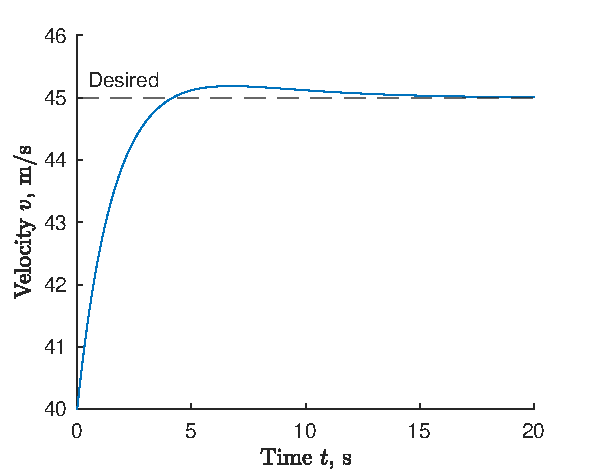
\includegraphics[height=0.8\textheight]{pdf/cruise-step}

\end{frame}

\begin{frame}
\frametitle{Cruise control phase portrait}
\centering
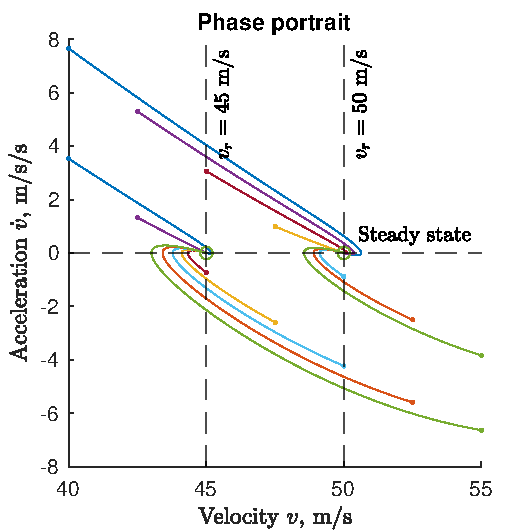
\includegraphics[height=0.8\textheight]{pdf/cruise-portrait}

\end{frame}

\SUBCONCEPT{Bicycle Dynamics}

\begin{frame}{Bicycle model}
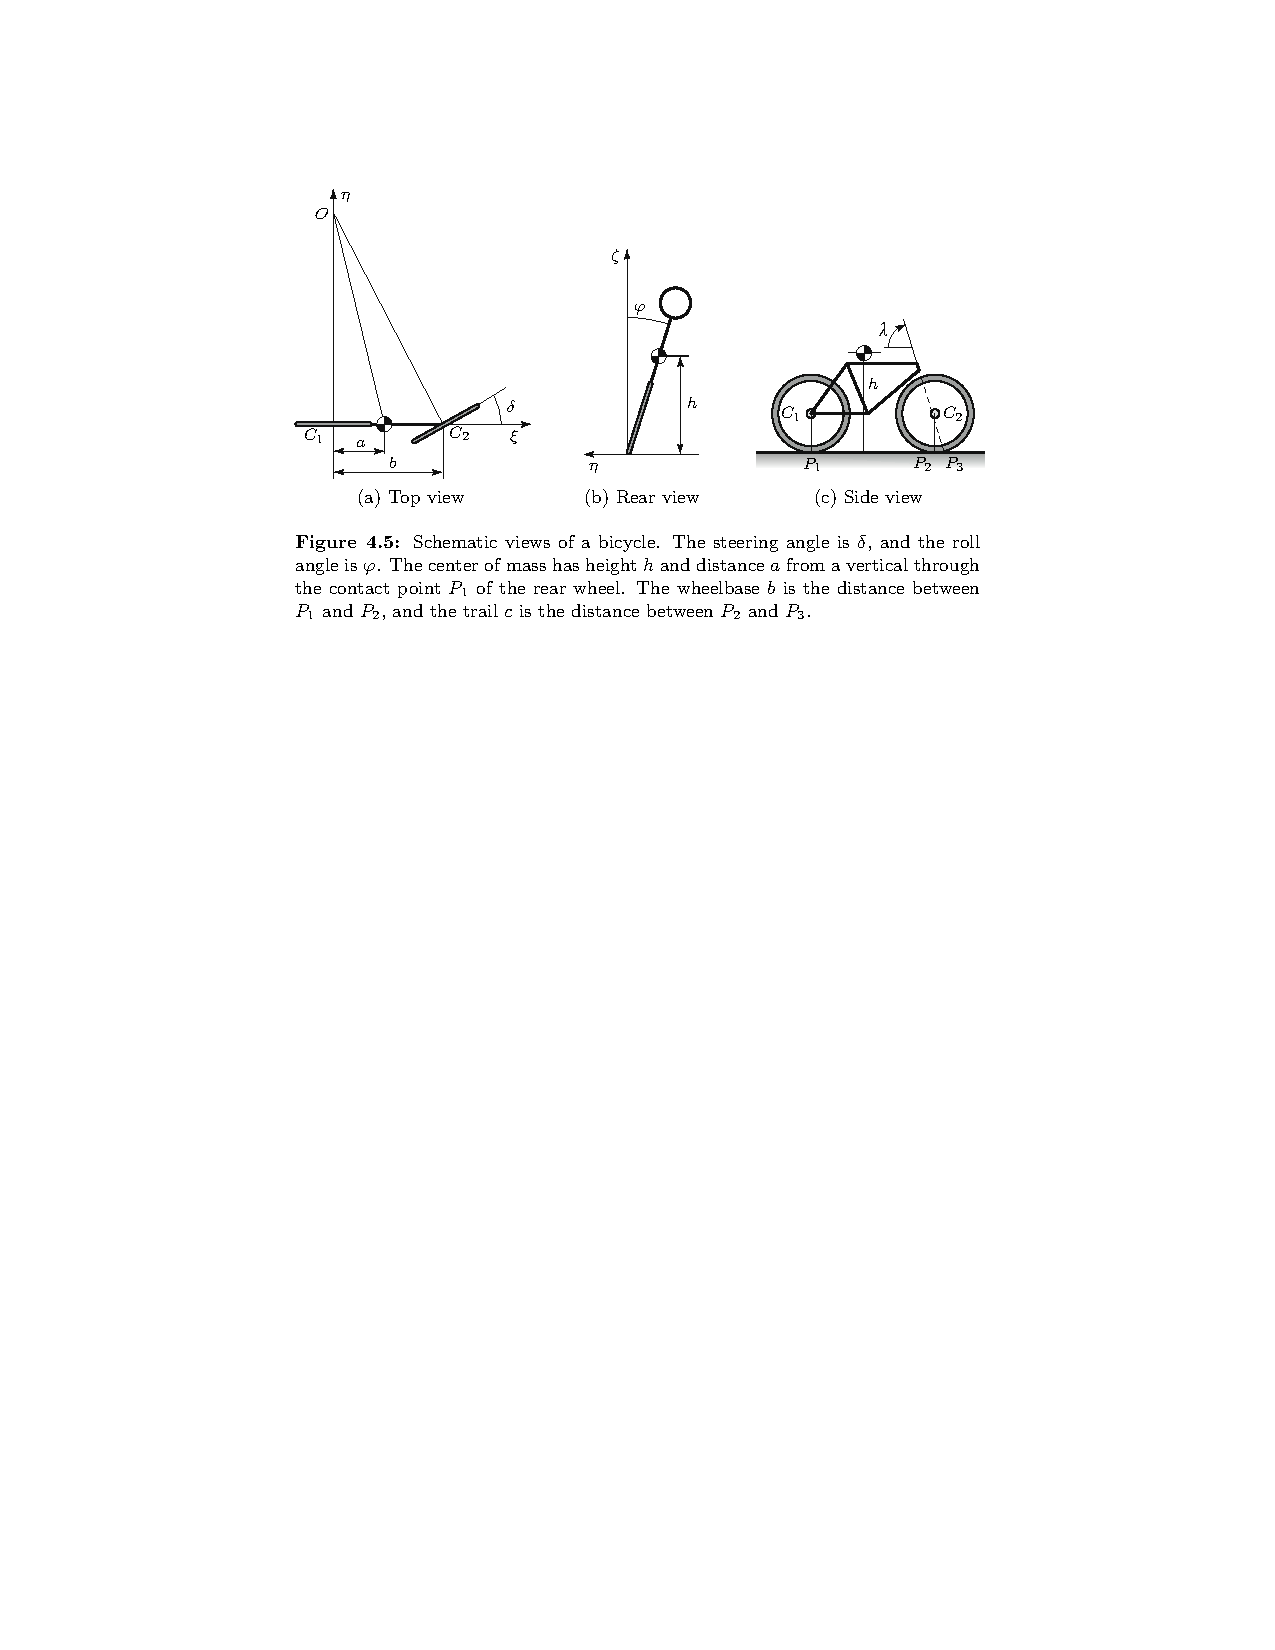
\includegraphics[width=\linewidth]{figure4.5}
\end{frame}

\begin{frame}{Bicycle dynamics}
\begin{uncoverenv}<1-2>
\begin{align}
J \Deriv{^2\varphi}{t^2} + \frac{Dv_0k_2}{b} \Deriv{\varphi}{t} + \left(\frac{mv_0^2hk_2}{b}-mgh\right)\varphi
&= \frac{Dv_0k_1}{b} \Deriv{T}{t} + \frac{mv_0^2hk_1}{b} T
\end{align}
\end{uncoverenv}
\begin{uncoverenv}<1>
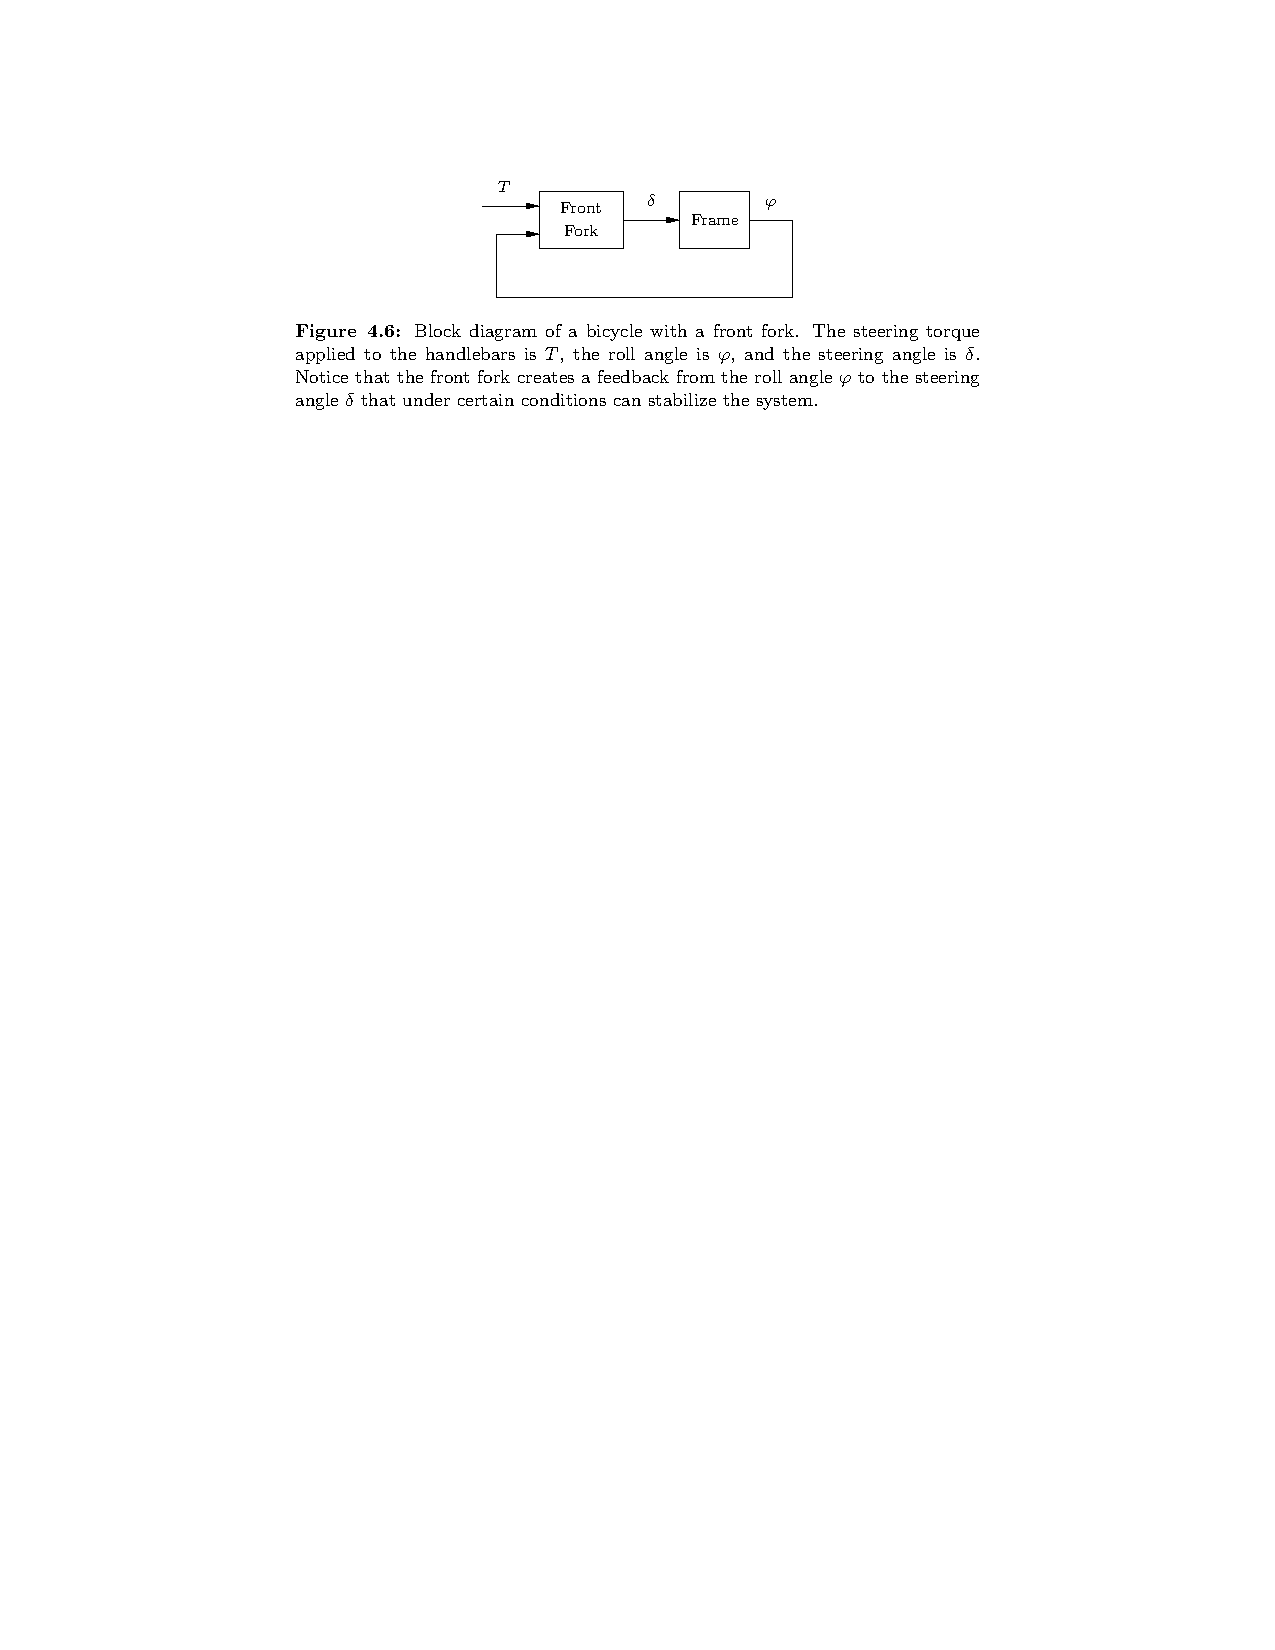
\includegraphics[width=\linewidth]{figure4.6}
\end{uncoverenv}

\end{frame}


\SUMMARYFRAME
\FINALE

\end{document}
